\section{Simuladores de realidad virtual}
\label{art:simulador}

\begin{figure}[h]
   \centering
    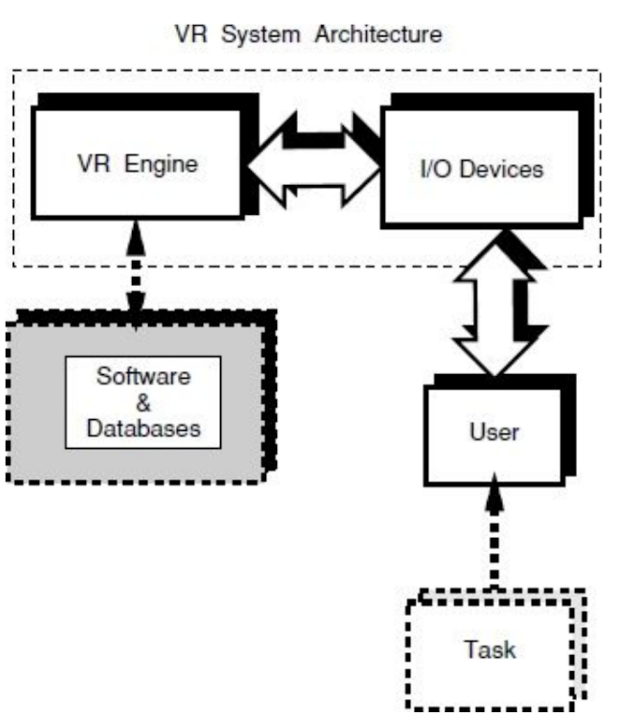
\includegraphics[width=0.5\textwidth]{IMG/VRarq.PNG}
    \caption{Arquitectura propuesta por \cite{burdea2003virtual}. }
   \label{fig:RVarq}
\end{figure}
Según \emph{Burdea y Coiffet}\cite{burdea2003virtual}, un sistema de \ac{RV} se puede dividir en cinco componentes tal y como se puede observar en la figura \ref{fig:RVarq}. En ella se puede observar las distintas interacciones que se producen entre los componentes. De manera separada, estos componentes pueden existir independientemente pero, es la relación que existe entre ellos, la que componen un sistema de \ac{RV}. A continuación, se describirá cada uno de ellos:
\begin{itemize}
    \item Motor de \ac{RV}: Este componente se encarga de realizar los cálculos necesarios para simular la escena virtual. Para actualizar el estado de la escena virtual, es necesario que se consulte las bases de datos y software incluidos en el sistema y actuar según la entrada recibida a través de los dispositivos realizada por los usuarios. El motor generará y mostrará el nuevo estado de la escena a través de los dispositivos de salida (que pueden incluir más de un canal sensorial). Además, es preciso asegurar una tasa interactiva al realizar estos cálculos. El término motor de RV no se puede asociar a un computador, sino que se tiene que tratar como una abstracción ya que puede tener múltiples configuraciones hardware como puede ser un único computador o un sistema distribuido conectado por red.
    \item Dispositivos de \ac{E/S}: Este componente se basa en todos los dispositivos que utilice el usuario en su interacción con el sistema. Es imprescindible en un sistema de \ac{RV}  permita la interacción del usuario. Los dispositivos de entrada se encargan de recoger las acciones que realiza el usuario, mientras que los dispositivos de salida muestran la respuesta de la escena virtual a través de los distintos canales sensoriales. Estos dispositivos son muy numerosos y diversos actualmente.
    \item Componentes software y base de datos: Este módulo contiene todas las especificaciones y descripciones que caracterizan el sistema. Aquí se incluyen la escena virtual y su organización que es consultada por el motor de \ac{RV} análogamente a lo que correspondería como una base de datos, donde se consulta y se recoge la información necesaria para la simulación. Además, aquí se incluyen, por ejemplo, las aplicaciones que se diseñan con el objetivo de guiar y facilitar el entrenamiento al dirigir la simulación según la interacción del sistema y el usuario.
    \item Usuario: Es natural que los sistemas se diseñen con el objetivo de que una persona interaccione con ellos. Esta comunicación se realizará a través de los dispositivos de \ac{E/S}. 
    \item Tareas: Por último, son las tareas, objetivos e instrucciones que se le dan al usuario cuando va a utilizar el sistema de \ac{RV} que le dan significado y utilidad al simulador. Es lo que le diferencia de ser un computador con periféricos conectados de una plataforma de entrenamiento para pilotos o médicos. 
    
\end{itemize}

Esta definición de arquitectura será utilizada en el capítulo \ref{cap:rasim} como apoyo para explicar el simulador \ac{RASim} y sus diferentes componentes. A su vez, también puede ayudar al lector a hacerse una idea de como se han construidos los simuladores que se presentarán en las siguientes secciones.

\subsection{Simuladores para formación médica}
\label{art:medicalsim}

En los últimos años, los simuladores médicos de realidad virtual están tomando una gran importancia en el currículum de los estudiantes, como pueden ser los cirujanos y otras especialidades \cite{PATEL2017266.e7}. Se puede observar un incremento de su presencia para el entrenamiento de jóvenes especialistas tanto en hospitales como universidades. Estas herramientas proporcionan al usuario un método seguro y efectivo de entrenamiento, siendo capaces de usarlo tantas veces como sea posible. 

Aunque los simuladores están cobrando cada vez más importancia, la enseñanza de medicina se basa en una variedad de métodos de entrenamiento que permite al médico adquirir las destrezas necesarias antes de poder enfrentarse a escenarios reales de manera autónoma. Una forma segura de entrenamiento es la utilización de \emph{fantomas}\cite{phantomra}. En la figura \ref{fig:phantom} se puede ver el \emph{Blue Phantom™}\cite{BluePH} para la práctica de ultrasonografía. Estos \emph{fantomas}\footnote{castellanización del término inglés Phantom} son modelos anatómicos hechos con materiales sintéticos intentando replicar el cuerpo humano fielmente y sus propiedades. En ocasiones, tienen incorporados una serie de sensores que permiten recogida de métricas. A pesar de que son muy populares, tienen una serie de inconvenientes: no son baratos, y suelen ser creados específicamente para una zona anatómica concreta, no siendo posible usarlos en otras circunstancias para lo que fueron creados. Además si, en determinadas ocasiones, el usuario tiene que manipularlos como puede ser hacer una incisión o realizar una inyección en el \emph{fantoma}, el modelo sufrirá desgaste con el tiempo.
\begin{figure}[h]
   \centering
    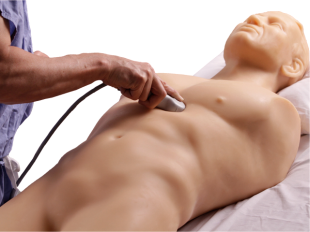
\includegraphics[width=0.5\textwidth]{IMG/fast_trauma.jpg}
    \caption{Maniquí realista para el entrenamiento de ultrasonografía  \emph{Blue Phantom™}\cite{BluePH}. }
   \label{fig:phantom}
\end{figure}

Otra forma de entrenamiento es la utilización de cadáveres\cite{Tsui2007}, que permiten una anatomía real en comparación con los \emph{fantomas}. En este caso, conseguir diferentes variaciones anatómicas es completamente viable y el mismo cadáver puede servir para entrenamientos de diferentes procedimientos. Aun así, los inconvenientes que presentan son bastante evidentes. Mantener un cadáver en buenas condiciones o que los motivos del fallecimiento hayan perjudicado al estado del mismo, además de ciertos problemas éticos como puede ser el uso de cadáveres procedentes de condenados a pena de muerte (Visible Human Project \cite{ackerman1998visible}). Finalmente, los tejidos de un cadáver no muestran el mismo comportamiento mecánico que un tejido vivo, y puede inducir sesgos en el entrenamiento del médico debido a que los músculos se vuelven más rígidos después del fallecimiento.


La última forma de entrenamiento es la práctica supervisada sobre pacientes reales, donde el estudiante realiza el procedimiento vigilado y guiado por su tutor. Aunque es el entrenamiento más realista, obviamente incluye una serie de riesgos y situaciones no controladas que pueden ser peligrosas para el paciente.


A diferencia de los métodos anteriormente citados, los simuladores de realidad virtual permiten un entrenamiento más barato y rápido donde los estudiantes pueden mejorar sus habilidades. Mejoras en el rendimiento, nuevos dispositivos de \ac{E/S} y el desarrollo de nuevas técnicas de simulación física, permiten una transferencia efectiva de habilidades del mundo virtual al mundo real. Habitualmente los simuladores  son específicos de cada procedimiento médico donde se pueden encontrar un simulador de cirugía ortopédica \cite{cecil2017advanced}, o por ejemplo un simulador de cirugía cardiovascular \cite{korzeniowski2018vcsim3}. Incluso, es posible combinar especialidades: \cite{villard2014interventional} es un simulador de radiología intervencional donde se entrena la habilidad quirurgica, además se puede practicar el guiado de la aguja a través de una imagen de rayos X.

Pero además, la nueva generación de simuladores no solo se centran en mejorar la calidad de la simulación. Existe la tendencia de permitir el entrenamiento incorporando datos de pacientes reales \cite{Willaert2012,  Votta2013}. 








